\documentclass[10pt, reqno]{amsart}
\usepackage[margin = 0.5 in]{geometry}
\usepackage{multicol}
\usepackage{float}
\usepackage{fancyhdr}
\usepackage{physics}
\usepackage{graphicx}
\usepackage{hyperref}
\usepackage{fancyvrb}
\usepackage{mathtools} 

\setlength{\abovecaptionskip}{5pt plus 3pt minus 3pt}

\hypersetup{colorlinks=true,allcolors=blue}
\pagestyle{fancy} \fancyhead{} \fancyfoot[C]{\normalsize\thepage}
\renewcommand{\headrulewidth}{0pt}
\begin{document}
\title{Vorticity-Streamfunction Solver Development \quad Jacob Ivanov}

\maketitle

\begin{multicols}{2}
\vspace{-.1 in}

\section*{Variable Declarations}
\begin{itemize}
\item $\vec{u}$ is the velocity vector, with $x$- and $y$-components of $u$ and $v$, respectively.
\item $k_p$ and $k_q$ are the $x$- and $y$-direction wavenumbers.
\item 
\end{itemize}

\section*{Integration Method}
In order to evalutate the governing equations of fluid evolution numerically, a Runge-Kutta method was employed, with the following Butcher Table:
\begin{equation}
    \begin{array}{c | cccc }
        0   & \\
        8/15 & 8/15 \\
        2/3 & 1/4 & 5/12 \\
        \hline
            & 1/4 & 0 & 3/4
    \end{array}
\end{equation}
Or an alternative representation:
% \begin{equation}
    \begin{gather}
    k_1 = f(t_n, u_n) \\
    k_2 = f \left(t_n + \frac{8 \Delta t}{15}, u_n + \frac{8\Delta t}{15}k_1 \right) \\
    k_3 = f \left(t_n + \frac{2 \Delta t}{3}, u_n + \Delta t \left( \frac{1}{4}k_1 + \frac{5}{12}k_2 \right) \right) \\
    u_{n+1} = u_n + \Delta t \left( \frac{1}{4} k_1 + \frac{3}{4} k_3 \right)
    \end{gather}
% \end{equation}
The autonomous version of this Runge-Kutta system is described in \textit{Spectral Methods for the Navier-Stokes Equations with one Infinite and two Periodic Directions} by Spalart et al. It is also known as the Van der Houwen, or Wray's Method.

This integration method was tested on the following ODE: 
\begin{equation}
    \begin{dcases}
        \frac{\dd y}{\dd t} = y \\
        y(t = 0) = 1
    \end{dcases}
\end{equation}
which has the recognizable solution $y(t) = e^t$.

\section*{Advection Transport Convergence}
The model advection PDE is as follows:
\begin{equation}
    \pdv{\theta}{t} + a \pdv{\theta}{x} + b \pdv{\theta}{y} = 0
\end{equation}
where $\theta$ is some type of scalar transport variable (ie temperature or species concentration). This type of first-order linear PDE can be analytically solved using the \href{https://en.wikipedia.org/wiki/Method_of_characteristics}{Method of Characteristics}, but here the solution will be given, and it is straightforward to use the Chain Rule for Multivariable Functions to show that it will satisfy the original PDE:
\begin{equation}
    \begin{cases}
        \theta(t, x, y) = f(x - at, y - bt) \\
        \theta(t = 0, x, y) = f(x, y)
    \end{cases}
\end{equation}
In other words, the solution is a translation of the initial conditions moving at speeds $a$, $b$ in the $x$-, $y$-directions, respectively.

However, as we numerically integrating this on a computational grid, we have to be mindful of numerical stability. In this case, the stability criterion for this advection model is the \href{https://en.wikipedia.org/wiki/Courant%E2%80%93Friedrichs%E2%80%93Lewy_condition}{Courant-Friedrichs-Lewy Condition}, which, applied to this problem is:
\begin{equation}
    \Delta t \left( \frac{a}{\Delta x} + \frac{b}{\Delta y} \right) \leq \mathrm{CFL}_\mathrm{max}
\end{equation}
where $\mathrm{CFL}_\mathrm{max}$ is dependent on the exact method.

\begin{figure}[H]
    \centering
    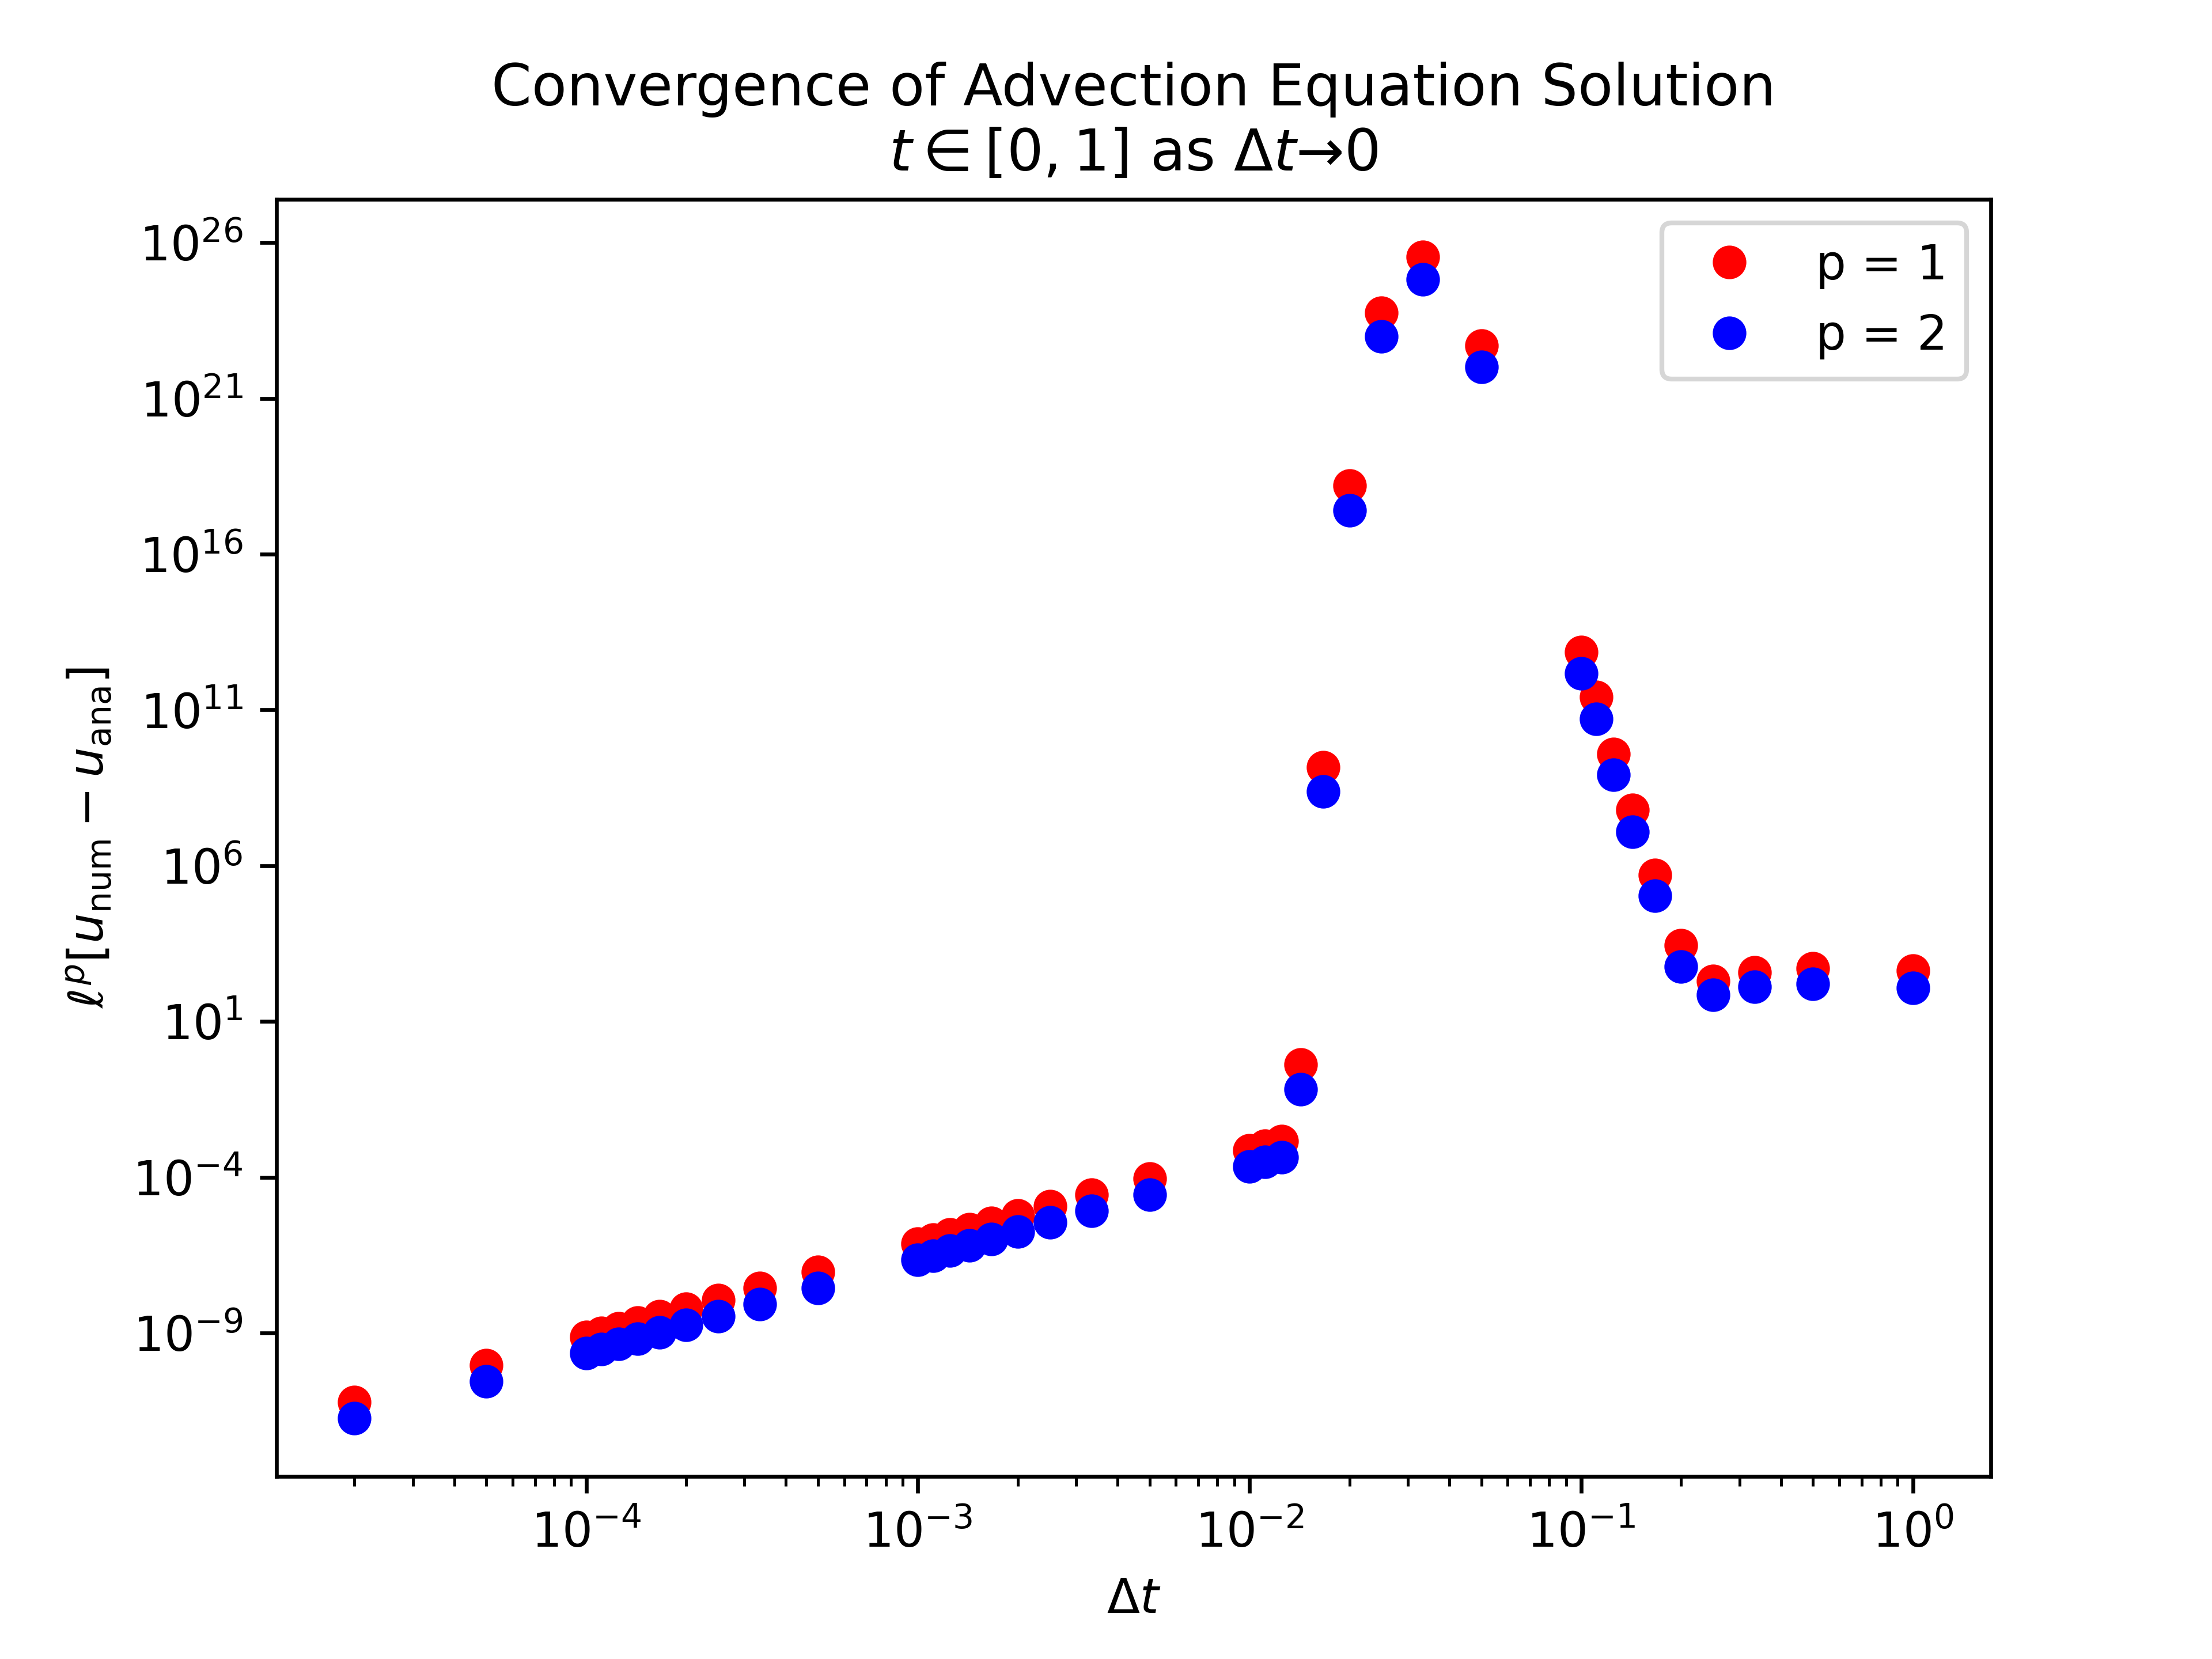
\includegraphics[width = 1\linewidth]{advection_convergence.png}
\end{figure}

\section*{Governing Equations}
The Navier-Stokes Equations for two dimensional, incompressible flow, in the absence of external body forces is as follows:
\begin{equation}
    \pdv{u}{t} + u \pdv{u}{x} + v \pdv{u}{y} = -\frac{1}{\rho} \pdv{p}{x} + \nu \left( \pdv[2]{u}{x} + \pdv[2]{u}{y} \right)
\end{equation}
\begin{equation}
    \pdv{v}{t} + u \pdv{v}{x} + v \pdv{v}{y} = -\frac{1}{\rho} \pdv{p}{y} + \nu \left( \pdv[2]{v}{x} + \pdv[2]{v}{y} \right)
\end{equation}
where $\vec{u} = \langle u, v \rangle$ is the velocity field, $p$ is the pressure field, and $\nu$ is the kinematic viscosity. By differentiating (1) with respect to $y$ and (2) with respect to $x$, and subtracting the resulting equations, we will eliminate pressure from the equation and can obtain the following:
\begin{equation}
    u = \pdv{\psi}{y}, \quad v = - \pdv{\psi}{x}
\end{equation}
\begin{equation}
    \pdv{}{t} \left[ \nabla^2 \psi \right] + \pdv{\psi}{y} \pdv{}{x} \left[ \nabla^2 \psi \right] - \pdv{\psi}{x} \pdv{}{y} \left[ \nabla^2 \psi \right] = \nabla^2 \left[ \nabla^2 \psi \right]
\end{equation}
The following relationship can be proven, where $\omega$ is the vorticity:
\begin{equation}
    \begin{aligned}
    \omega &= \nabla \times \vec{u} = \pdv{v}{x} - \pdv{u}{y} \\
    &= - \nabla^2 \psi = \pdv{}{x} \left[ - \pdv{\psi}{x} \right] - \pdv{}{y} \left[ \pdv{\psi}{y} \right]
    \end{aligned}
\end{equation}
As a result, (4) can be re-written as follows:
\begin{equation}
    \pdv{\omega}{t} = \nu \left( \pdv[2]{\omega}{x} + \pdv[2]{\omega}{y} \right) - \left(u \pdv{\omega}{x} + v \pdv{\omega}{y} \right)
\end{equation}
Here we need to clarify notation. Lowercase variables represent values in physical space, and uppercase in frequency space. Similarly, subscript indices $i, j$ correspond to physical space, and $p, q$ correspond to frequency space. By using discrete spectral methods, equation (6) can be re-written as:
\begin{equation}
    \pdv{\Omega_{pq}}{t_n} = - \nu \left(k_p^2 + k_q^2 \right) \Omega_{pq} - \mathcal{F}^2 \left[ u_{ij} \pdv{\omega_{ij}}{x_i} + v_{ij} \pdv{\omega_{ij}}{y_j} \right]
\end{equation}
We can now introduce an integrating factor as follows:
\begin{equation}
    \Xi_{pq}(t_n) = \exp \left( \nu \left(k_p^2 + k_q^2 \right) t_n \right)
\end{equation}
\begin{equation}
    \pdv{}{t_n} \left[ \Xi_{pq} (t_n) \cdot \Omega_{pq} \right] = - \mathcal{F}^2 \left[ u_{ij} \pdv{\omega_{ij}}{x_i} + v_{ij} \pdv{\omega_{ij}}{y_j} \right]
\end{equation}
Due to the incompressibility assumption, the right hand side of (9) can be manipulated to:
\begin{equation}
    \begin{aligned}
    \pdv{}{t_n} \left[ \Xi_{pq} (t_n) \cdot \Omega_{pq} \right] &= - \underline{i} \Xi_{pq}(t_n) \cdot \left( k_p \cdot \mathcal{F}^2 \left[ u_{ij} \omega_{ij} \right] \right. \\
    & \left. + k_q \cdot \mathcal{F}^2 \left[ v_{ij} \omega_{ij} \right] \right)
    \end{aligned}
\end{equation}

\section*{Integrating Factor Modification}
It can be seen in Eq. 8 that $\partial \Xi_{pq} / \partial t$ is strictly positive. As a result, as time $t_n$ increases, particularly for larger computational grid sizes, our numerical evaluation for $\Xi_{pq}$ becomes first, decreasingly precise, then overflows due to the 64 bit double floating-point format that it stored as. However, we can exploit the exponential form of $\Xi_{pq}$ to modify Eq. 10 to become the following:
\begin{equation}
    \begin{aligned}
    \pdv{}{t_n} \left[ \Xi_{pq}(\tau) \cdot \Omega_{pq} \right] &= - \underline{i} \Xi_{pq}(\tau) \cdot \left( k_p \cdot \mathcal{F}^2 \left[ u_{ij} \omega_{ij} \right] \right. \\
    & \left. + k_q \cdot \mathcal{F}^2 \left[ v_{ij} \omega_{ij} \right] \right)
    \end{aligned}
\end{equation}
where $\tau$ is calculated for each Runge-Kutta substep as $\tau = t - t_n$. As a result, we reduce the effect of floating point innacuracies in $\Xi_{pq}$ and eliminate the possibility of overflows.

\section*{Stablized Forcing Method}
We will define a new wavenumber array: 
\begin{equation}
    k_\Xi = \begin{cases}
        k_p^2 + k_q^2 \\
        k_p
    \end{cases}
\end{equation}

\section*{Particle Transport}
Consider a point particle dropped into a flow. If the particle is non-inertial, it will instantaneouly be travelling at the same velocity and direction as the flow surrounding it.
\begin{equation}
    \vec{v}(t, \vec{x}_p) = \vec{u}(t, \vec{x}_p)
\end{equation}
where $\vec{x}_p$ is the particle position vector, $\vec{u}$ is fluid velocity vector, and $\vec{v}$ is the particle velocity vector. As a result, the particle position can be directly found by integrating the fluid velocity, as follows:
\begin{equation}
    \vec{x}_p = \int_0^t \left[ \vec{v}(t, \vec{x}_p) \right] \dd t
\end{equation}

As the Streamfunction positions in unperturbed Taylor-Green Flow are time-invariant, ie.
\begin{equation}
    \psi(t, x, y) = - \frac{1}{\beta} e^{-2 \nu t} \cos(\beta x) \cos(\beta y)
\end{equation}
We can perform a test to this method by calculating the Modified Streamfunction, $\psi_0$ at the particle position for each timestep. 
\begin{equation}
    \psi_0(x, y) = \frac{1}{\beta} \cos(\beta x) \cos(\beta y)
\end{equation}
\begin{figure}[H]
    \centering
    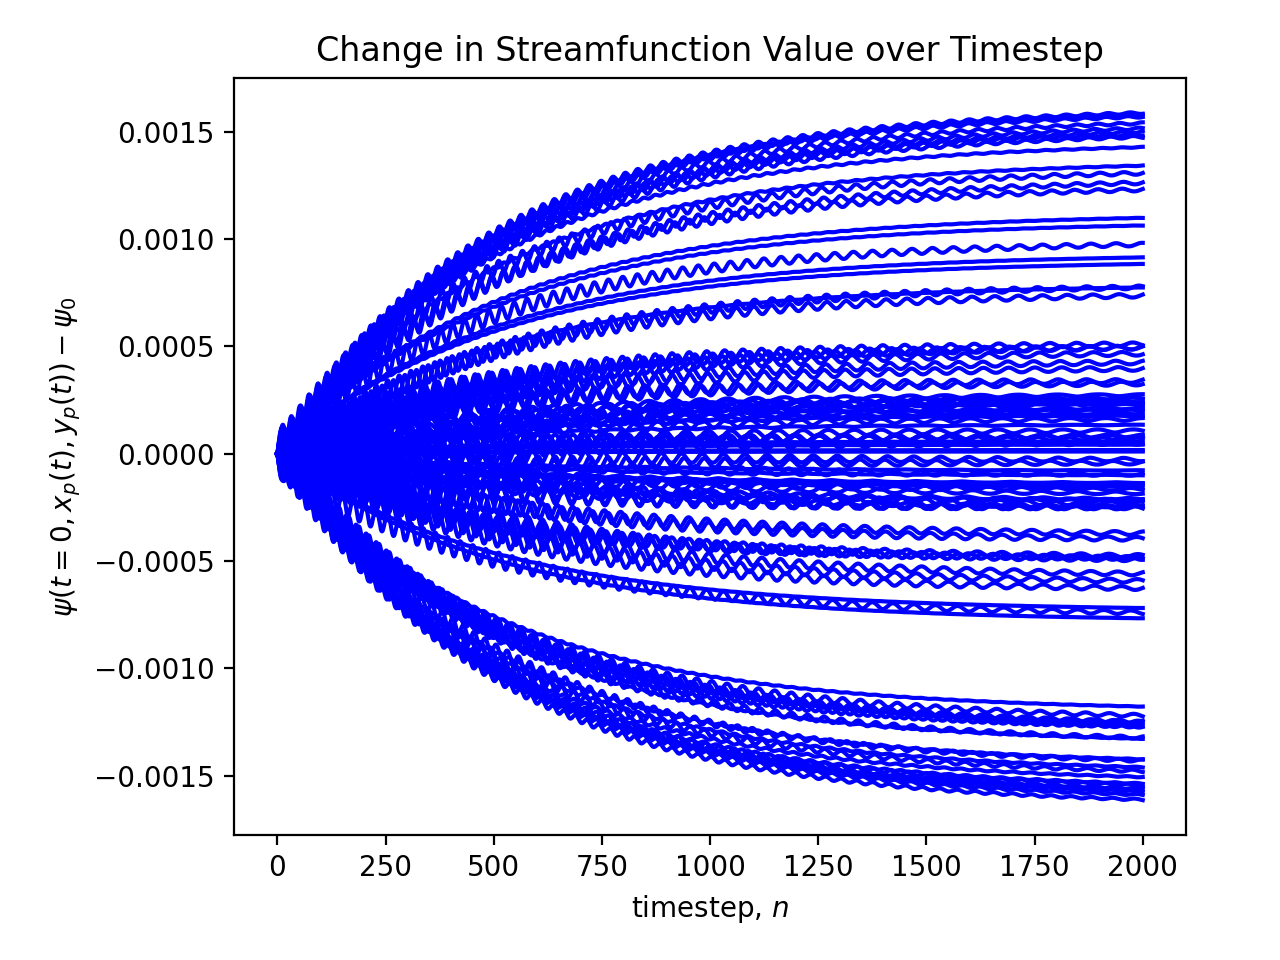
\includegraphics[width = 1\linewidth]{Predictor-Corrector TG 100 Trajectories.png}
\end{figure}
With a function range of $ -1 \leq \psi_0(x, y) \leq +1$, and  $\max |\Delta \psi_0| \approx 0.0015$ over 2000 timesteps of $\Delta t = 0.1$, it can be seen that this error is very well controlled.

If the particle is inertial, we can define a non-dimensional inertial time, $\tau$, which is depedent on the particle geometry and fluid viscosity. For our purposes, we will just consider it to be an independent constant. The particle velocity is related to the fluid velocity by the following Coupled ODE:
\begin{equation}
    \frac{\dd \vec{v}}{\dd t} = \frac{1}{\tau} (\vec{u} - \vec{v}) + 3 \frac{\dd \vec{u}}{\dd t}
\end{equation}
In the case of a known spatially-invariant fluid velocity field, $\vec{u}(t)$, the system has the following integro-differential solution (refer to Appendix B for the full derivation):
\begin{equation}
    \vec{v}(t) = e^{-t/\tau} \int_0^t e^{\lambda/ \tau} \left[ \frac{u(\lambda)}{\tau}  + 3 \frac{\dd}{\dd \lambda} \Big[ u(\lambda) \Big] \right] d \lambda
\end{equation}
\begin{equation}
    \vec{x}_p(t) = \int_0^t [\vec{v}(t)] \dd t
\end{equation}
However, in the case of a spatially-varying fluid velocity field, we then have to rely on numerical methods. The following Predictor-Corrector Scheme was utilized. Starting with an initial $\vec{x}_n$, $\vec{u}_n$, and $\vec{v}_n$:

\begin{equation}
    \vec{x}_{n + \alpha} = \vec{x}_n + \Delta t \cdot \vec{v}_n
\end{equation}
\begin{equation}
    \vec{u}_{n + \alpha} = \vec{u}(\vec{x}_{n + \alpha}, t_{n + 1})
\end{equation}
\begin{equation}
    \vec{v}_{n + \alpha} = \frac{\vec{v}_n + \Delta t \left[ \vec{u}_{n + \alpha}/\tau + 3 \vec{a}_n \right]}{1 + \Delta t/\tau}
\end{equation}
\begin{equation}
    \vec{x}_{n+1} = x_n + \frac{\Delta t}{2} (\vec{v}_n + \vec{v}_{n + \alpha})
\end{equation}
\begin{equation}
    \vec{u}_{n+1} = \vec{u}( \vec{x}_{n+1}, t_{n+1} )
\end{equation}
\begin{equation}
    \vec{a}_{n+1} = \vec{a}( \vec{x}_{n+1}, t_{n+1} )
\end{equation}
\begin{equation}
    \begin{aligned}
    \vec{v}_{n+1} &= \frac{1}{1 + \frac{\Delta t}{2 \tau}} \Bigg[ \vec{v}_n + \Bigg. \\ 
    & \Bigg. \frac{\Delta t}{2} \left( 3 ( \vec{a}_n + \vec{a}_{n+1} ) + \frac{\vec{u}_n + \vec{u}_{n+1} - \vec{v}_n}{\tau} \right) \Bigg]
    \end{aligned}
\end{equation}
This whole Predictor-Corrector Scheme degenerates to Heun's Method for the non-inertial case.


\section*{Appendix A: Spectral Differentiation}
Consider a 1D discretized function $T(x_i) = T_i$. Through the use of the Fourier Transform, we can see that (note that $\underline{i} = \sqrt{-1}$):
\[ T_i = \sum_p \left[ \hat{T}_p \cdot e^{- \underline{i} k_p x_i} \right] \]
\[ \left. \frac{\dd T}{\dd x} \right|_i = \sum_p \left[- \underline{i} k_p \hat{T}_p \cdot e^ {- \underline{i} k_p x_i} \right] = \sum_p \left[ \frac{\dd  \hat{T_p}}{\dd x} \cdot e^ {- \underline{i} k_p x_i} \right] \]

\[ \left. \frac{\dd T}{\dd x} \right|_i = \text{ifft} \left[ \underline{i} k_p \cdot \hat{T}_p \right] \]
It follows that:
\[ \left. \frac{\dd ^2T}{\dd x^2} \right|_i = \text{ifft} \left[ -1 k_p^2 \cdot \hat{T}_p \right ] \]

\section*{Appendix B}
\[ \frac{\dd v}{\dd t} = \frac{1}{\tau} (u - v) + 3 \frac{\dd u}{\dd t} \]
\[ \frac{\dd v}{\dd t} + \frac{1}{\tau} v = \frac{1}{\tau} u + 3 \frac{\dd u}{\dd t} \]
\[ \frac{\dd}{\dd t} \left[ \mu v \right] = \frac{\mu}{\tau} u + 3 \mu \frac{\dd u}{\dd t} \quad \mathrm{ where } \quad \mu = \exp \left[ \int \frac{1}{\tau} \dd t \right] = e^{t/\tau} \]
\[ \mu v = \int \left[ \frac{\mu}{\tau} u + 3 \mu \frac{\dd u}{\dd t} \right] \dd t \]
\[ v(t) = e^{-t/\tau} \int_0^t \left[ e^{\lambda / \tau}{\tau} u(\lambda) + 3e^{\lambda / \tau} \frac{\dd}{\dd \lambda} \left[ u(\lambda) \right] \right] d \lambda \]
\end{multicols}
\end{document}